\subsection{Rapidity}

Uma variável útil de se definir em um estudo de colisões de partículas a velocidades relativísticas é a {\it rapidity} $y$. Mas antes,
definimos o conceito de massa transversa.
\par
Toda colisão de partículas possui um eixo específico, chamdo eixo de colisão. Associado a este eixo, há um plano transverso. As componentes
dos momentos no eixo da colisão e no plano transverso serão identificadas como $p_{L}$ e $p_{T}$, respectivamente. Essas variáveis podem ser
melhor compreendidas observando a Figura \ref{fig:geometria}.

\begin{figure}[!h]
 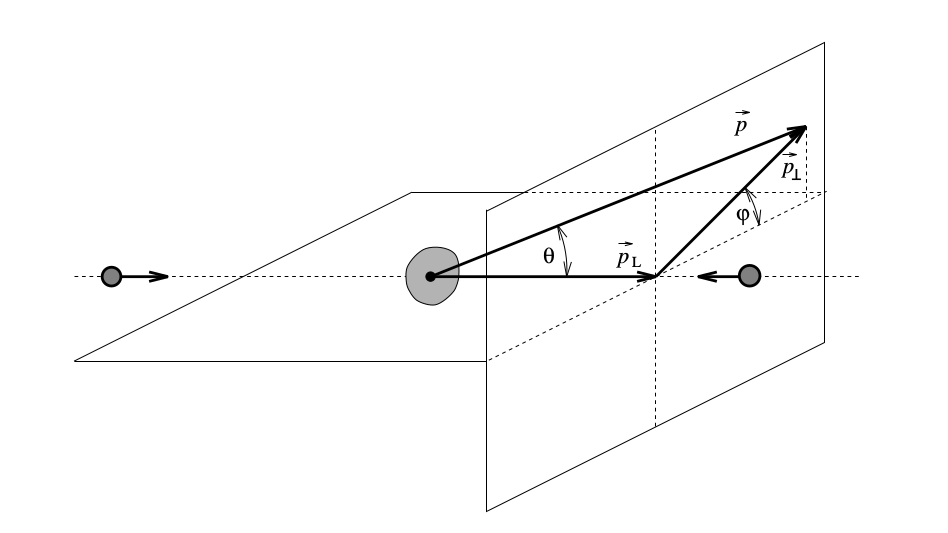
\includegraphics[scale=0.35]{Content/geometriamomento.png}
 \caption{Ilustração geométrica de $p_T$ e $p_L$.}
 \label{fig:geometria}
\end{figure}


Associada ao momento transversal, definimos a massa transversa:

\begin{equation}
 m_{T}=\sqrt{m^2+p_{T}^2}
\end{equation}

Ao contrário de $p_{L}$, $p_{T}$ não depende do referencial em que a colisão é estudada, portando, é uma boa variável. É necessário, então,
definir uma variável no eixo de colisão, esta será a {\it rapidity}. Definimos esta através das equações:

\begin{subequations}
\begin{align}
 E=m_{T} \cosh{(y)} \\ p_{L}=m_{T} \sinh{(y)}
\end{align}
\end{subequations}

Isolando $\eta$ nas equações acima obtemos:

\begin{equation}
 y = \ln{(\frac{E+p_{L}}{m_{T}})}
\end{equation}

Uma propriedade importante desta variável, é que ela é aditiva em relação a transformações de Lorentz.

\subsection{Pseudorapidity}

Quando a energia de uma partícula é muito grande comparada à sua massa, podemos escrever:

\begin{equation}
\begin{split}
 y   & = \ln{\frac{E+p_{L}}{m_{T}}} \\
     & = \frac{1}{2}\ln{\frac{(E+p_{L})^2}{m_{T}^2}} \\
     & = \frac{1}{2}\ln{\frac{(E+p_{L})^2}{E^2-p_{L}^2}} \\
     & = \frac{1}{2}\ln{\frac{E+p_{L}}{E-p_{L}}} \\
     & \approx \frac{1}{2}\ln{\frac{p+p_{L}}{p-p_{L}}} \\
     & \approx \frac{1}{2}\ln{\frac{1+\cos(\theta)}{1-\cos(\theta)}} \\
     & \approx \frac{1}{2}\ln{\cot{2\theta}} \\
\end{split}
\end{equation}

Definimos então, a variável {\it pseudorapidity}:

\begin{equation}
 \eta = \frac{1}{2}\ln{\cot{2\theta}}
\end{equation}

